\begin{frame}{RLHF --- Reinforcement Learning with Human Feedback}
  \begin{center}
    \Large
    RLHF --- Reinforcement Learning with\\ Human Feedback
  \end{center}
\end{frame}


\begin{frame}[t]{Why RLHF?}
  \begin{itemize}
    \item[\textcolor{red}{$\blacktriangleright$}] SFT doesn't teach the model what humans prefer.
    \item[\textcolor{red}{$\blacktriangleright$}] RLHF introduces reward learning and policy optimization.
    \item[\textcolor{red}{$\blacktriangleright$}] Inspired by InstructGPT (Ouyang et al., 2022).
  \end{itemize}
\end{frame}

\begin{frame}{RLHF Pipeline Overview}
  \begin{enumerate}
    \item \textbf{Supervised Fine-Tuning (SFT):} Train the base model on instruction-response pairs.
    \item \textbf{Reward Model (RM) Training:} Learn a reward function from human preference rankings.
    \item \textbf{RL Optimization (e.g., PPO):} Optimize the language model to maximize the learned reward.
  \end{enumerate}
\end{frame}


\begin{frame}{RLHF Pipeline}
  \begin{figure}
    \centering
    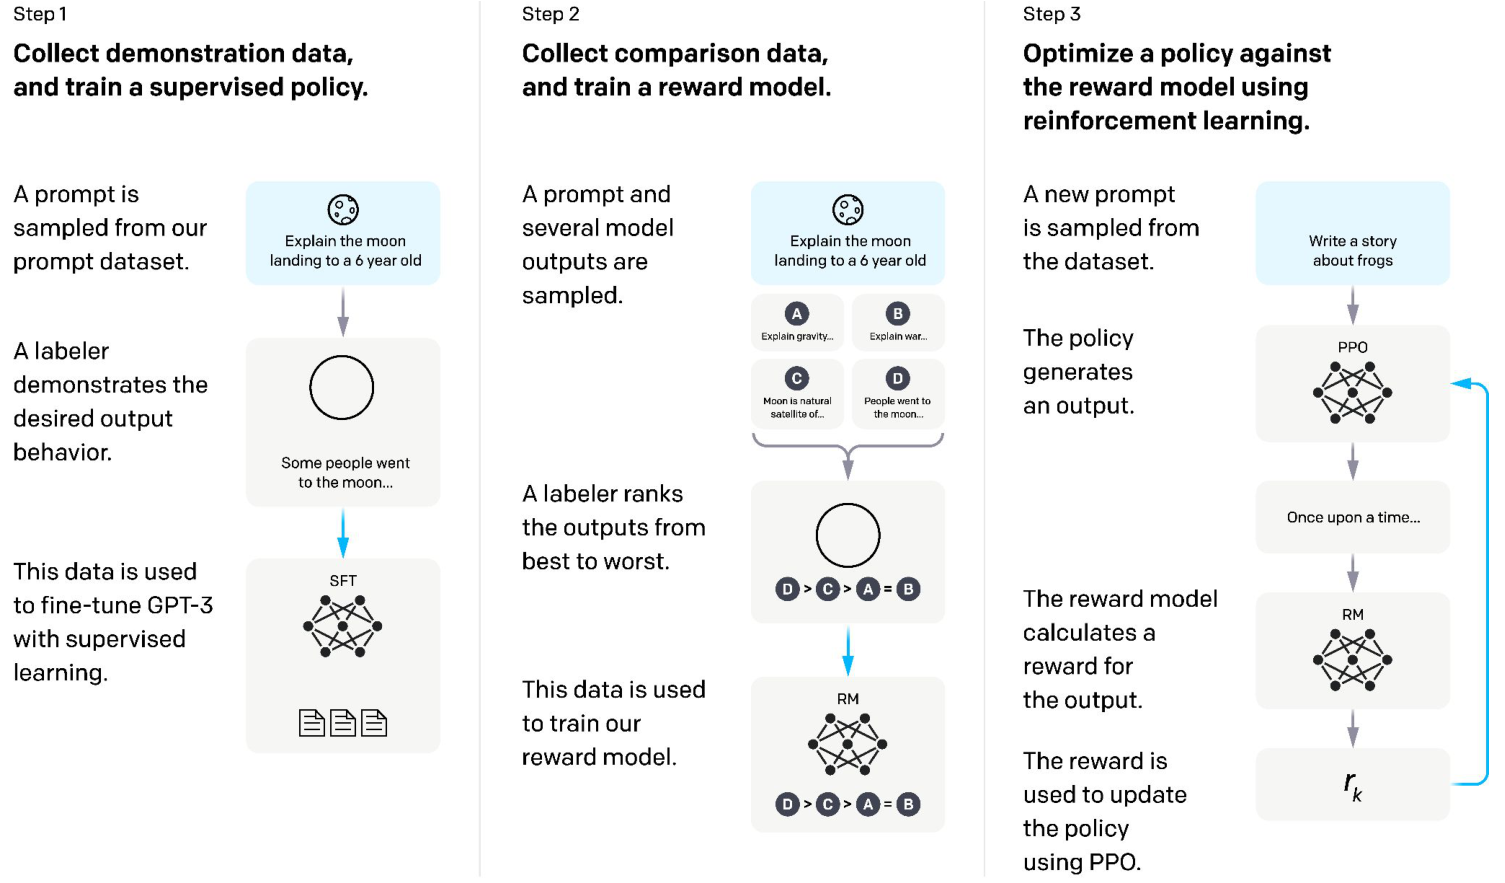
\includegraphics[width=0.76\paperwidth,height=0.60\paperheight,keepaspectratio]{images/llm-rlhf/rlhf_three_step_pipeline.png}
    \caption*{\scriptsize Ouyang et al., ``Training language models to follow instructions with human feedback,'' NeurIPS 2022, Fig.~2.}
  \end{figure}
\end{frame}

\begin{frame}{RLHF Pipeline}
  \begin{figure}
    \centering
    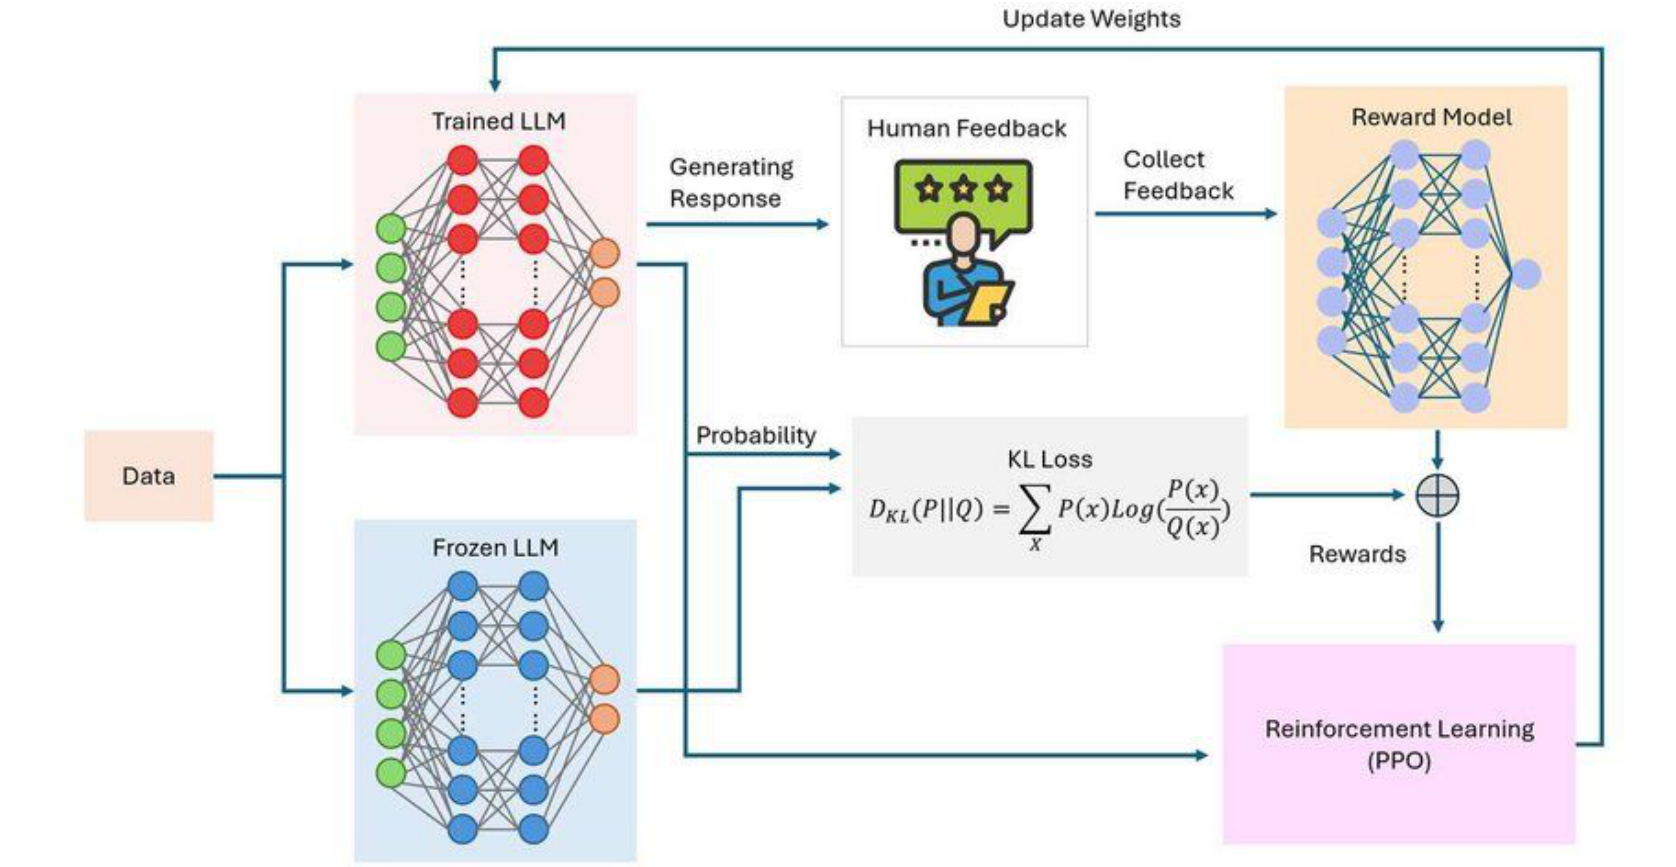
\includegraphics[width=0.60\paperwidth,height=0.60\paperheight,keepaspectratio]{images/llm-rlhf/rlhf_training_loop_diagram.png}
    \caption*{\scriptsize Source: Wu, You \& Du, ``AI generations: from AI 1.0 to AI 4.0,'' \textit{Frontiers in Artificial Intelligence} 8:1585629, 2025, Fig.~7.}
  \end{figure}
\end{frame}
